\chapter{\IfLanguageName{dutch}{Stand van zaken}{State of the art}}%
\label{ch:stand-van-zaken}

% Tip: Begin elk hoofdstuk met een paragraaf inleiding die beschrijft hoe
% dit hoofdstuk past binnen het geheel van de bachelorproef. Geef in het
% bijzonder aan wat de link is met het vorige en volgende hoofdstuk.

% Pas na deze inleidende paragraaf komt de eerste sectiehoofding.

Zoals in hoofdstuk \ref{ch:inleiding} werd vermeld, wordt er een oplossing gezocht voor het slim aansturen van bepaalde bedrijfsprocessen van het bedrijf Carwash Clean Car. Voordat er oplossingen kunnen worden besproken, is het belangrijk dat er een grondige voorkennis wordt opgedaan over het onderwerp. Deze literatuurstudie zal daarbij helpen. Om tot een geschikte oplossing te komen, is de literatuurstudie opgedeeld in 3 delen. In afbeelding \ref{fig:voorlopige-proefopstelling} wordt de voorlopige versie van de proefopstelling weergegeven, zodat een idee kan gevormd worden over hoe alles zal samenwerken.

\begin{figure}[h!]
    \centering
    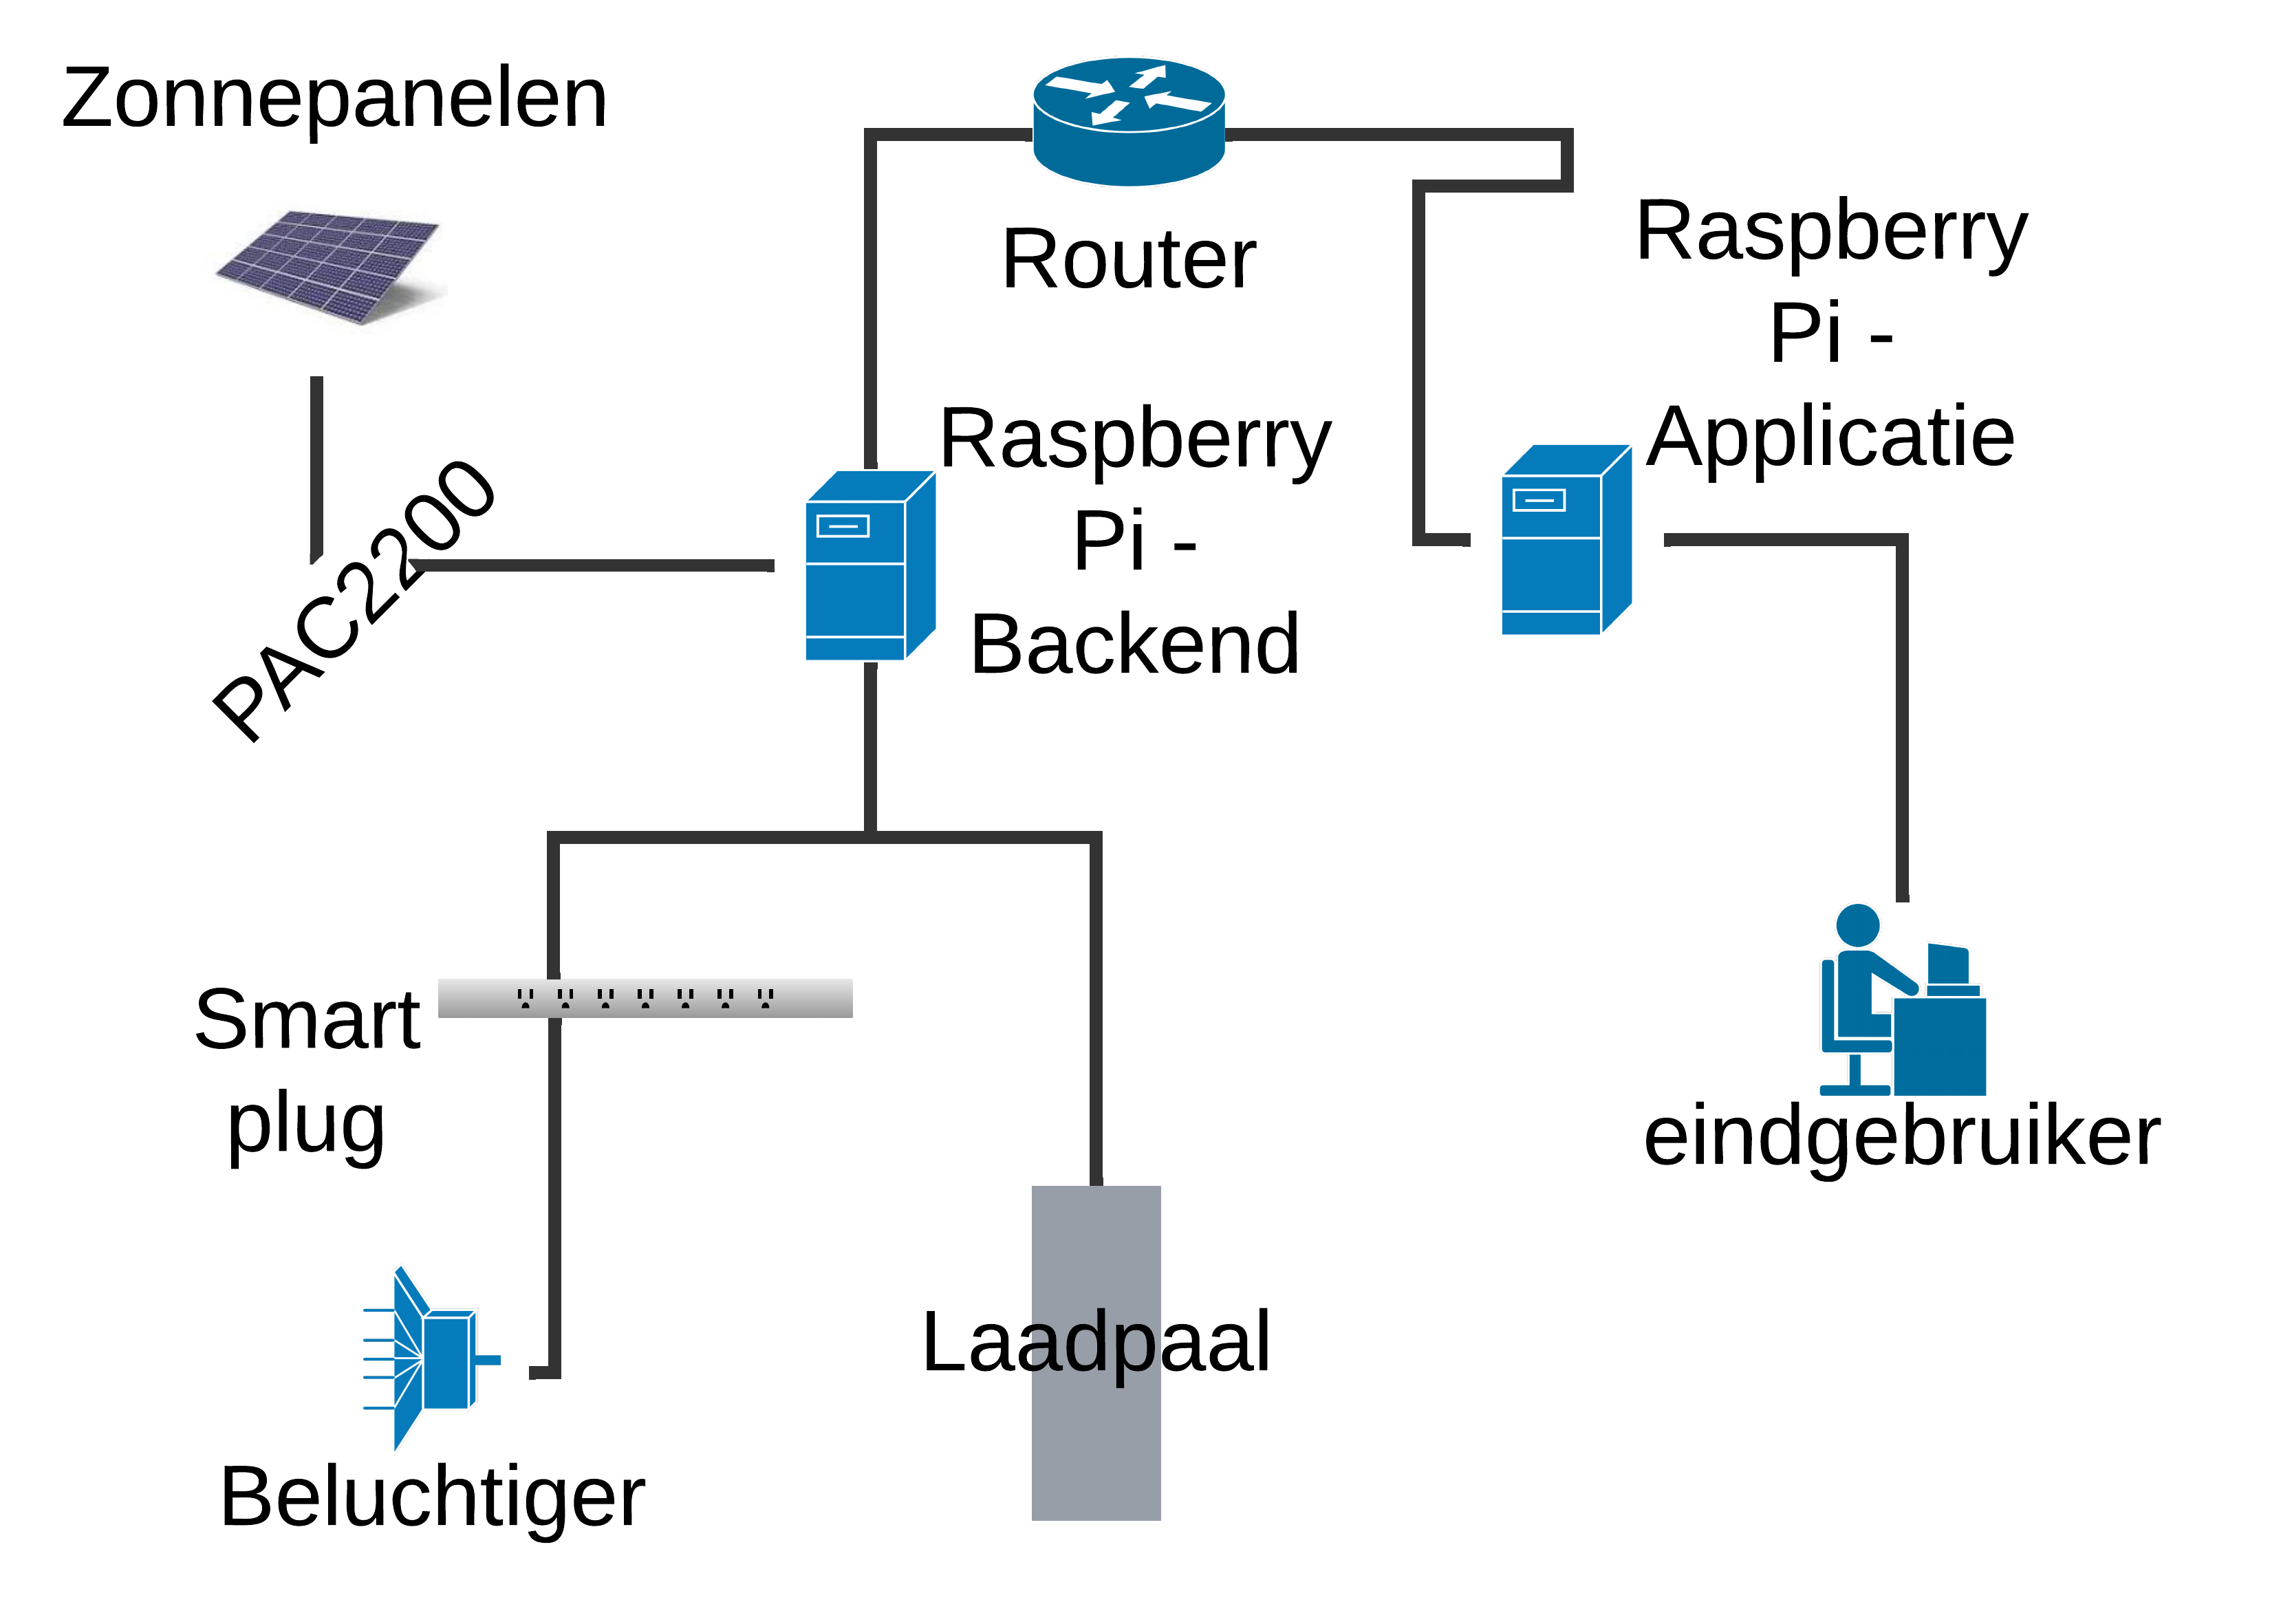
\includegraphics[width=20em]{./graphics/voorlopige-proefopstelling.png}
    \caption{Voorlopige illustratie van de proefopstelling}
    \label{fig:voorlopige-proefopstelling}
\end{figure}

Er zijn verschillende componenten aanwezig in afbeelding \ref{fig:voorlopige-proefopstelling}, deze componenten kunnen later nog wijzigen of er kunnen nog componenten bij komen, waardoor dit diagram niet meer klopt. De huidige componenten in het schema van afbeelding \ref{fig:voorlopige-proefopstelling} zijn:

\begin{itemize}
    \item De zonnepanelen
    \item De Siemens PAC2200
    \item De beluchter
    \item De smarplug waar de beluchter op aangesloten is
    \item De laadpaal
    \item 2 Raspberry Pi’s
    \begin{itemize}
        \item 1 Raspberry Pi voor de backend
        \item 1 Raspberry Pi voor de webapplicatie
    \end{itemize}
    \item De router
    \item De eindgebruiker
\end{itemize}

\section{Energieverbruikers van carwash Clean Car}
\label{sec:stand-van-zaken-energieverbruikers}

Aangezien deze casus zich richt op een carwash, is 1 van de belangrijkste energieverbruikers de machines en infrastructuur die gebruikt wordt om de tunnel van de carwash aan te sturen. De tunnel kan opgedeeld worden in 2 delen, het eerste deel dient voor het wassen van de auto’s, wat gemiddeld 5 kilowatt verbruikt per auto. Het tweede deel van de tunnel zorgt voor het drogen van de auto’s, dit verbruikt gemiddeld 50 kilowatt per auto. In de tunnel kunnen er 5 auto’s tegelijk gewassen worden, waarvan 1 van die auto’s in het deel voor het drogen is. Aangezien het wasproces niet altijd opnieuw moet opstarten, verbruikt de carwash op dat moment gemiddeld 55 kilowatt.\\

Naast deze tunnel is er ook nog de self carwash, die op het domein gevestigd is. De infrastructuur van deze self carwash hoort dan ook bij de belangrijkste energieverbruikers van het bedrijf. De selfcarwash bestaat uit 5 wasboxen. Als 1 box in gebruik is, wordt 1 pomp geactiveerd en wordt er 2 kilowatt verbruikt. Voor de 5 wasboxen tegelijk, wordt het verbruik dus 10 kilowatt.\\

Na de 2 belangrijkste energieverbruikers zijn er ook verschillende niet-dringende energieverbruikers, zo staat er een laadpaal geïnstalleerd, deze laadpaal wordt gebruikt voor het opladen van elektrische voertuigen. Het laadvermogen van de laadpaal kan zelf ingesteld worden tot een maximum vermogen van 11 kilowatt.\\

De tweede niet-dringende energieverbruiker is het beluchtingssysteem van het water, dit systeem is nodig om te voorkomen dat er algen ontstaan in het zelf gerecycleerde water in de waterputten. Het beluchtingssysteem heeft een vermogen van 3 kilowatt. Deze 3 kilowatt fluctueert niet, wat betekent dat het beluchtingssysteem continu 3 kilowatt verbruikt wanneer deze ingeschakeld wordt. Het systeem is niet continu ingeschakeld om schuimvorming te voorkomen.\\

De laatste energieverbruiker die besproken wordt is de industriële droogkast, deze droogkast wordt gebruikt voor het drogen van de werkkledij en de microvezeldoeken die gebruikt worden bij dieptereinigingen. De reden dat deze droogkast besproken wordt is omdat deze al verouderd en energie-intensief is. De droogkast is tot nu toe het niet-dringende bedrijfsproces met het hoogste verbruik. Het energieverbruik is namelijk 14 kilowatt.\\

De tunnel en self carwash worden in de proefopstelling niet aangesproken, omdat deze niet zomaar uitgeschakeld mogen worden. De industriële droogkast wordt na deze bachelorproef pas toegevoegd aan de proefopstelling, de oorzaak hiervan is dat de componenten om de droogkast slim aan te sturen nog besteld moeten worden. Al de rest van de besproken niet-dringende bedrijfsprocessen zullen wel al geïntegreerd worden met webapplicatie. 

\section{Peak shaving}
\label{sec:stand-van-zaken-peak-shaving}

Het eerste concept dat besproken wordt is peak shaving. De bedoeling van dit concept is om pieken in de aankoop van energie af te vlakken, dit kan gebeuren door bepaalde bedrijfsprocessen te verplaatsen naar momenten waar er minder energie verbruikt wordt of er te veel energie geïnjecteerd wordt op het energienet. Deze methode zorgt voor een meer gelijkvormige verdeling van het energieverbruik.\\

Er zijn verschillende methoden om peak shaving te bereiken, 1 mogelijke techniek die bij peak shaving gebruikt wordt volgens \textcite{UDDIN2018} is het gebruik van een energieopslagsysteem. Om deze methode te gebruiken zijn er batterijen nodig die energie kunnen opslaan, deze batterijen stellen het energieopslagsysteem voor. Volgens \textcite{UDDIN2018} kan deze methode peak shaving bereiken door batterijen op te laden wanneer de vraag naar elektriciteit laag is, ook wel een dalperiode genoemd. Deze methode kan economische voordelen opleveren voor het bedrijf, omdat tijdens de hoge vraag naar elektriciteit de batterijen gebruikt kunnen worden.

\section{Bidirectioneel laden van batterijen}
\label{sec:stand-van-zaken-bidirectioneel-laden}

1 van de concepten die aan het opkomen is bij laadpalen is bidirectioneel laden. Dit betekent dat, als een auto opgeladen wordt, deze auto batterij gebruikt kan worden om energie op te slaan voor later gebruik. Wat betekent dat de wagen ook energie kan teruggeven via de laadpaal. Dit zou handig zijn om niet-dringende bedrijfsprocessen aan te sturen als er energie aangekocht wordt. Dit concept kan ook toegepast worden op reserve batterijen die geïnstalleerd worden voor als de elektriciteit wegvalt.\\

Voor het gebruik van bidirectioneel laden van een auto is er een elektrische auto en een laadpaal nodig die dit ondersteunt. Er zijn al verschillende bedrijven die dit concept toepassen op hun wagens. Hoewel de wagen in de opstelling, een ID.Buzz van Volkswagen, bidirectioneel laden ondersteunt, kan dit nog niet in de proefopstelling benut worden omdat de laadpaal niet over deze functionaliteit beschikt.\\

Het verschil tussen een laadpaal die de functie van bidirectioneel laden niet heeft en een laadpaal die de functie wel heeft is het type van elektrische stroom dat de laadpaal gebruikt, zo bestaan er twee types van elektrische stroom namelijk wisselstroom (AC) en gelijkstroom (DC) \footnote{Deze informatie is op 6 mei 2024 teruggevonden op deze website: \url{https://www.vlaanderen.be/een-elektrische-wagen-laden/uw-elektrische-wagen-als-thuisbatterij}.}.\\

Bidirectioneel laden kan voor 2 toepassingen worden gebruikt, namelijk Vehicle-to-Grid (V2G) en Vehicle-to-Home (V2H), volgens \textcite{LAZZERONI2019} is vehicle-to-grid bedoeld voor het verkopen van opgeslagen energie aan het energienet. Terwijl vehicle-to-home daarentegen bedoeld is om de opgeslagen energie later zelf thuis te gebruiken.\\

Het interessantste voor het bedrijf is de vehicle-to-home oplossing, omdat als de elektriciteit wegvalt, er kan overgeschakeld worden op de batterij van de ID. buzz of reserve batterijen. Het voordeel hiervan is dat de elektriciteit niet moet wegvallen om de batterij van de ID. buzz te gebruiken, waardoor als er enkel energie aangekocht wordt er andere niet-dringende bedrijfsprocessen hiermee verder kunnen worden aangestuurd. De reden dat er niet voor de vehicle-to-grid oplossing gekozen wordt is omdat het bedrijf minder elektriciteit wil injecteren op het energienet, aangezien hier bijna niets aan verdiend wordt. In dit specifieke geval wordt er ingezet op het optimaliseren van het eigen verbruik en het minimaliseren van de injectie.

\subsection{Batterijen uit elektrische voertuigen}
\label{sec:stand-van-zaken-bidirectioneel-laden-batterijen}

Elk elektrisch voertuig heeft een batterij, deze batterij is nodig om te kunnen rijden. Zo zijn er verschillende batterijen beschikbaar waaruit de fabrikanten van de voertuigen kunnen kiezen, 4 van deze batterijen zijn:

\begin{itemize}
    \item Lithium-ion (Li-ion) batterij
    \item Loodaccu
    \item Nikkel-cadmium (NiCd) batterij
    \item Nikkel-metaalhydride (NIMH) batterij
\end{itemize}

In de volgende 5 paragrafen worden de bovenstaande batterijen besproken, de informatie in deze paragrafen komt van \textcite{AnupKumarH2022}, de Lithium-ion batterij werd begin jaren 90 uitgevonden. Deze uitvinding was een doorbraak op het gebied van batterijen, aangezien deze batterij efficiënter te werk gaat dan alle andere batterijen. Dit type van batterij wordt in veel draagbare elektronische apparaten gebruikt zoals in mobiele telefoons, laptops, …\\

Omdat de lithium-ion batterij een hoge energie-eenheid massa heeft, wordt deze batterij gekozen als batterij in de meeste elektrische voertuigen. Een paar eigenschappen van deze batterij zijn dat de batterij licht in gewicht is en een laag zelfontlading niveau heeft, wat betekent dat ze geen energie ontladen in rusttoestand. Een ander voordeel is dat de batterij met een minimum aan afval kan worden gerecycled.\\

De loodaccu werd uitgevonden door de Fransman Gaston Planté in 1860. Deze batterij werd tot in de jaren 80 gebruikt bij elektrische voertuigen, maar deze technologie is verdwenen met de komst van de Lithium-ion batterij. Zo zijn de loodaccu’s zwaarder en hebben deze een lagere energiedichtheid tegenover de Lithium-ion batterijen. De loodaccu’s worden wel nog gebruikt voor toepassingen met een laag vermogen en voor noodstroomvoorziening.\\

Hoewel de nikkel-cadmium batterij een exceptionele energiedichtheid en hoge efficiëntie had, hadden deze batterijen een lage levensduur. Deze batterij werd in 1899 uitgevonden en had marktdominantie tot het begin van de jaren 90. Ondanks deze dominantie wordt er geen voorkeur gegeven aan deze batterij voor het gebruik in moderne elektrische voertuigen. In de jaren 90 werden deze batterijen gebruikt in elektrische voertuigen, maar werden al snel verboden vanwege hun giftigheid.\\
Een aangepaste versie van nikkel-cadmium batterijen zijn de nikkel-metaalhydride batterijen, deze batterijen werden in 1989 gepatenteerd. De batterijen worden gebruikt in mild hybride voertuigen dat geen externe bron nodig heeft om op te laden. Ze kunnen enkel opgeladen worden door het regeneratieve remmechanisme. Dit remmechanisme zet kinetische energie om in warmte tijdens het remmen, deze warmte wordt dan gebruikt om de batterij op te laden.

\subsection{Wat is de impact van bidirectioneel laden?}
\label{sec:stand-van-zaken-bidirectioneel-laden-impact}

"De impact van bidirectioneel laden op de batterijen van elektrische voertuigen is een belangrijk aandachtspunt bij de ontwikkeling van smart grid-technologieën" \autocite{Dubarry2017}. \textcite{Elvan2017} en \textcite{Monteiro2013} stellen beide oplossingen voor dit probleem voor, waarbij Elvan een modulaire enkelfasige bidirectionele EV-lader met optimalisatie van de stroomdeling voorstelt en Monteiro het ontwerp van een bidirectionele batterijlader voor EV's bespreekt. Deze oplossingen zijn bedoeld om de efficiëntie en integratie van EV-laders in het slimme elektriciteitsnet te verbeteren. \textcite{Anuja2024} draagt verder bij aan dit gebied door een bidirectionele lader voor EV-toepassingen voor te stellen, die een bidirectionele DC-DC-omvormer bevat voor stroomregeling en netstabiliteit.

\section{Algoritmen}
\label{sec:stand-van-zaken-algoritmen}

Om de niet-dringende bedrijfsprocessen slim aan te sturen, kunnen er verschillende algoritmen gebruikt worden. Deze algoritmen worden bepaald aan de hand van de voorwaarden die opgelegd zijn door de eigenaar van het bedrijf. De basisvoorwaarden die bij carwash Clean Car opgelegd zijn, zijn dat de niet-dringende bedrijfsprocessen enkel mogen aangestuurd worden als er meer energie opgewekt wordt dan dat er verbruikt wordt. Als een bedrijfsproces overdag niet aangestuurd is geweest, wordt deze in de nacht uitgevoerd.\\

Er zijn verschillende soorten algoritmen die aan de hand van de basisvoorwaarden gebruikt kunnen worden, zoals:

\begin{itemize}
    \item een algoritme voor het bepalen van de prioriteit van bedrijfsprocessen
    \item een algoritme voor het optimaal gebruik van bedrijfsprocessen
    \item een algoritme voor de inschakeling van bedrijfsprocessen
\end{itemize}

Deze 3 algoritmen zijn de algoritmen waarmee de proefopstelling van start gaat. Het kan zijn dat deze algoritmen nog geoptimaliseerd worden of er nog algoritmen bij komen doorheen de testfase van de proefopstelling.

\subsection{Het algoritme voor het bepalen van de prioriteit van bedrijfsprocessen}
\label{sec:stand-van-zaken-algoritme-prioriteit}

Dit algoritme zal aan elk bedrijfsproces een prioriteit toekennen, deze prioriteit zal bepaald worden aan de hand van de laatste keer dat het bedrijfsproces aangestuurd is geweest en de energie die het bedrijfsproces verbruikt. Hoe langer het geleden is dat het bedrijfsproces aangestuurd is geweest, hoe hoger de prioriteit zal zijn. Als er meerdere bedrijfsprocessen zijn die even lang geleden aangestuurd zijn geweest, zal de prioriteit bepaald worden aan de hand van het energieverbruik van het bedrijfsproces.

\subsection{Het algoritme voor het optimaal gebruik van bedrijfsprocessen}
\label{sec:stand-van-zaken-algoritme-optimaal}

Dit algoritme zal een lijst teruggeven met bedrijfsprocessen die aangestuurd kunnen worden bij het huidige overschot van energie. Deze lijst wordt bepaald aan de hand van de prioriteit van het bedrijfsproces en zal zo het meeste aantal energie van het huidige overschot van energie in gebruik nemen, zodat de energie zo min mogelijk verspilt wordt.

\subsection{Het algoritme voor het aansturen van bedrijfsprocessen}
\label{sec:stand-van-zaken-algoritme-aansturen}

Dit algoritme zal gebruikt worden voor het in en uitschakelen van bedrijfsprocessen. Dit gebeurt aan de hand van de laatste lijst die gegenereerd is met het algoritme voor het optimaal gebruik van bedrijfsprocessen.

\section{energiebeheersysteem}
\label{sec:stand-van-zaken-energiebeheersysteem}

Dit is een systeem voor het beheren en monitoren van de energie die verbruikt wordt binnen het bedrijf. Volgens \textcite{FALOPE2024} kunnen energiebeheersystemen opgedeeld worden in 2 groepen, namelijk voorspellende energiebeheersystemen en realtime energiebeheersystemen.\\

In de volgende paragraaf wordt het verschil tussen de 2 groepen van energiebeheersystemen aangehaald aan de hand van de paper van \textcite{FALOPE2024} een voorspellend energiebeheersysteem maakt gebruik van historische data om een belasting voorspelling, een energievoorziening voorspelling of een combinatie van beide te genereren. Deze voorspellingen zorgen ervoor dat het energieaanbod optimaal overeenstemt met de vraag naar energie. Omdat voorspellingen echter niet 100~\% wetenschappelijk ondersteund zijn, moet er als een reserve methode de realtime planning van de energiebelasting geïntegreerd worden in een voorspellend energiebeheersysteem om voorspellingsfouten aan te passen. Een realtime energiebeheersysteem daarentegen, zal gebruikmaken van algoritmen om de regeling van de energiebelasting of energielevering aan te passen.\\

Het verschil tussen de twee groepen is de aanpak voor het weergeven van de energiebelasting en energielevering om zo de bedrijfsprocessen aan te sturen. Aangezien er niet genoeg data beschikbaar is om een voorspellend energiebeheersysteem te creëren, zal er een realtime energiebeheersysteem gebruikt worden.

\section{Laadpaal voor de elektrische voertuigen}
\label{sec:stand-van-zaken-laadpaal}

Het laden van de bedrijfswagens is 1 van de niet-dringende bedrijfsprocessen van Carwash Clean Car. Voor dit bedrijfsproces uit te voeren, heeft het bedrijf 1 laadpaal staan om de 2 bedrijfswagens op te laden. De 2 wagens in kwestie zijn een Volkswagen ID. Buzz en een Volvo XC90 T8. De Volkswagen ID. Buzz is een volledig elektrische wagen, de XC90 daarentegen, is een plug-in hybride wagen. De laadpaal die gebruikt wordt bij het bedrijf is de Eve Single S-line van het merk Alfen. Deze laadpaal is gekozen omdat deze slim aangestuurd kon worden en dat de laadpaal aangesloten kon worden op krachtstroom, in vlaanderen ook wel drijfkracht genoemd. Dit betekend dat de elektriciteit geleverd wordt met een spanning van 400 volt in plaats van 230 volt\footnote{Deze informatie is op 18 mei 2024 teruggevonden op deze website: \url{https://www.woorden.org/woord/krachtstroom}.}.\\

Volgens \textcite{HEMAVATHI2022} zijn er 2 connector types bij laadpalen, namelijk AC connectoren en DC connectoren. Deze 2 types hebben zelf ook nog elk hun eigen onderverdeling. Zo bestaat er binnen de familie van AC connectoren de onderverdeling binnen type 1 en type 2. Het type 1 is de SAE J1772 standaard. Dit type is de standaard in Amerika en Azië en kan tot 7,4 kilowatt snel laden. Het andere type is de IEC 62196-2 standaard dat gebruikt wordt in Europa. Dit type kan tot 43 kilowatt snel laden. Er zijn 3 DC connectoren, namelijk de CHAdeMO, de CCS en de Tesla connectors. De CHAdeMO connector is uitgevonden in Japan en kan een laadsnelheid bereiken tot 100 kilowatt. Het CCS, kort voor Combined Charging System, is een combinatie van een type 2 AC connector en DC connector. De AC connector kan tot 43 kilowatt en de DC connector tot 100 kilowatt snel laden. De laatste connector is de Tesla connector, deze connector maakt gebruik van de 480 volt snellaad technologie met een maximum oplaadsnelheid van 250 kilowatt. Deze technologie zorgt ervoor dat een auto volledig opgeladen kan worden in 1 uur tijd. \\

De laadpaal van Carwash Clean Car heeft een AC type 2 connector, maar is beperkt tot een laadsnelheid van 11 kilowatt. Volgens de datasheet van Alfen\footnote{Deze informatie is op 6 mei 2024 teruggevonden op deze website: \url{https://alfen.com/nl-be/file-download/download/public/2753}.} komt de geïnstalleerde laadpaal al met verschillende slimme laad functies, zoals active load balancing, ook wel dynamic load balancing genoemd. Dit houdt in dat de laadpaal actief het stroomverbruik in de gaten houdt, zodat deze zo het laadvermogen aanpast voor de laadpaal.\footnote{Deze informatie is teruggevonden op 6 mei 2024 op deze website: \url{https://www.elix.nl/load-balancing-alles-wat-je-moet-weten/}.} Uiteindelijk bleek dit niet te werken hoe de eigenaar van Carwash Clean Car dit bedoelde. De uitbater wilde dat de laadpaal ingeschakeld werd wanneer er meer zonne-energie is dan dat er gebruikt wordt, dus de laadpaal moet ingeschakeld worden als er 11 kilowatt of meer geproduceerd wordt. De reden dat dit niet werkt is omdat, vanaf er meer zonne-energieproductie is, dan energie dat gebruikt wordt, de waarde op de energiemeter negatief is. De oplossing hiervoor is zelf de laadpaal aan te spreken, dit kan door 1 van de ingang protocollen aan te spreken die beschikbaar zijn op de laadpaal, deze protocollen zijn:

\begin{itemize}
    \item DSMR 4.0-4.2 en SMR5.0
    \item Externe relais
    \item Modbus TCP/IP (externe kilowattuur meter)
    \item Modbus TCP/IP Slave (energiebeheersysteem)
    \item Modbus RTU (externe kilowattuur meter)
    \item Télé-information client (slimme meter linky)
\end{itemize}

Het protocol dat aangesproken zal worden is het Modbus TCP/IP Slave protocol. Dit komt doordat de webapplicatie die ontwikkeld wordt een energiebeheersysteem is. Zo kan er aan de hand van een prioriteits algoritme bekeken worden of laadpaal ingeschakeld mag worden.

\section{Zonnepanelen}
\label{sec:stand-van-zaken-zonnepanelen}

De zonnepanelen van carwash Clean Car zijn geplaatst om de maandelijkse energiefactuur te verlagen. Sinds begin 2022 merkt het bedrijf op dat op momenten dat de infrastructuur van de carwash niet actief is, er veel energie geïnjecteerd wordt op het energienet. Als de zonneproductie beperkt is en de infrastructuur van de carwash plus de niet-dringende energie-intensieve bedrijfsprocessen actief zijn, valt op dat dan wel energie aangekocht moet worden, dit zorgt er dan weer voor dat de maandelijkse energiefactuur te duur wordt.\\

Het bedrijf heeft in totaal 432 ET-Solar zonnepanelen op hun domein. Het piekvermogen van 1 paneel bedraagt 235 wattpiek, dus als alle panelen samen hun volledige capaciteit benutten, bedraagt het piekvermogen 101 520 wattpiek. De gemiddelde opbrengst van 06/05/2023 tot en met 06/05/2024 bedraagt 149,01 kilowatt. Om de opgewekte zonne-energie om te zetten naar elektriciteit zijn er omvormers nodig, hiervoor maakt de carwash gebruik van deze omvormers:

\begin{itemize}
    \item ABB Trio 27,6 TL (2x geïnstalleerd)
    \item SMA Tripower 15000 TL (1x geïnstalleerd)
    \item SMA Tripower 17000 TL (1x geïnstalleerd)
\end{itemize}

Voor het uitlezen van de hoeveelheid energie die opgewekt wordt met de zonnepanelen bij het bedrijf zijn er 2 apparaten die geïnstalleerd zijn en gebruikt kunnen worden. Zo kan de opgewekte energie geraadpleegd worden via De Solarlog 1000 van Solarinventors. Het nadeel van de Solarlog 1000 is dat het enkel de opgewekte energie meet en niet de aangekochte energie of het verbruik van energie, maar hier heeft de eigenaar een energiemonitor voor geïnstalleerd, namelijk de Siemens PAC2200. Deze energiemonitor kan het huidige verbruik en aangekochte energie monitoren. De combinatie van de 2 apparaten zorgt ervoor dat alle factoren, zoals het huidige energieverbruik, de huidige opwekking van energie en de energie die geïnjecteerd wordt op het energienet, kunnen geraadpleegd worden.\\

Om het apparaat van Solarlog te integreren met de applicatie, zal deze uitgelezen moeten worden. Aangezien het Modbus TCP protocol op dit apparaat geïnstalleerd staat, zal dit protocol gebruikt moeten worden voor het uitlezen van de opgewekte energie. Als de opgewekte energie uitgelezen is kan deze data weergeven worden aan de hand van een grafiek die eens de data wijzigt geüpdatet wordt.\\

Voor het aanspreken van de Siemens PAC2200 zijn er verschillende protocollen beschikbaar. De ondersteunde communicatieprotocollen van dit apparaat zijn teruggevonden bij de subtitel Ethernet onderaan pagina 28 van de handleiding van Siemens van dit product\footnote{Deze informatie is op 17 april 2024 teruggevonden op deze website: \url{https://cache.industry.siemens.com/dl/files/681/109476681/att_108732/v1/SITRANS_PAC2200_UM_EN-US_A6V1020.pdf}.}:

\begin{itemize}
    \item Modbus TCP
    \item Web Server (HTTP)
    \item SNTP
    \item DHCP
\end{itemize}

Aangezien er data verkregen moet worden, kunnen er 3 van deze protocollen niet gebruikt worden, namelijk de webserver, het SNTP protocol en het DHCP protocol. Om de data te verkrijgen zal dus het Modbus TCP protocol gebruikt moeten worden. In sectie \ref{sec:stand-van-zaken-protocollen} wordt er dieper ingegaan op het Modbus protocol.

\section{Beluchtingssysteem van het water}
\label{sec:stand-van-zaken-beluchtingssysteem}

Het bedrijf carwash Clean Car zuivert een deel van het water dat er gebruikt wordt in de carwash zelf, voor dit proces is er een beluchtingssysteem geïnstalleerd. Dit beluchtingssysteem verbruikt continu 3 kilowatt en moet niet de hele dag actief zijn, hierdoor wordt dit proces momenteel enkel in de nacht uitgevoerd. Dit bedrijfsproces moet minimaal 30 minuten per 24 uur aanstaan. Daarom kwam de vraag of deze beluchter ook smart aangestuurd kan worden aan de hand van een smart plug.\\

Voor het beluchtingssysteem slim aan te sturen is er een smart plug voorzien, deze smart plug zal verbonden zijn met het internet om aangestuurd te kunnen worden. Via de webapplicatie zal er een booleaanse waarde doorgestuurd worden naar de backend. De backend zal dan op zijn beurt, aan de hand van de booleaanse waarde, een signaal doorsturen naar de smart plug om deze aan of af te zetten.\\

De benodigdheden voor het automatisch aansturen van de smart plug is niet veel, namelijk een smart plug met internetverbinding en een applicatie voor het aansturen ervan is voldoende. Het aansturen zelf gebeurt aan de hand van een booleaanse waarde. Aan de hand van deze booleaanse waarde zal de backend het juiste signaal doorsturen naar de smart plug om deze in of uit te schakelen.\\

\section{Industriële droogkast}
\label{sec:stand-van-zaken-droogkast}

De industriële droogkast is een van de niet-dringende bedrijfsprocessen die nog niet geïntegreerd is in de proefopstelling. Dit bedrijfsproces wordt gebruikt om de werkkledij van de eigenaar en de microvezeldoeken die de eigenaar gebruikt voor dieptereinigingen. De reden hiervoor is dat het component dat nodig is om de droogkast slim aan te sturen nog besteld moet worden. 1 van de redenen dat de droogkast geïntegreerd moet worden in de proefopstelling is omdat deze droogkast verouderd en energie-intensief is. Het component dat nog nodig is om deze droogkast slim aan te sturen is een smart plug.

\section{protocollen}
\label{sec:stand-van-zaken-protocollen}

Aangezien er verschillende protocollen nodig zijn voor de apparaten, zoals de zonnepanelen en de laadpaal aan te spreken, worden deze hier uitgebreider besproken. De reden hiervoor is dat er een grondige voorkennis wordt opgedaan over de protocollen die gebruikt kunnen worden.\\

De protocollen die gebruikt gaan worden zijn versies van het Modbus protocol. Zo wordt voor de zonnepanelen Modbus TCP/IP gebruikt en voor laadpaal zal Modbus TCP/IP Slave connectie gebruikt worden.\\

"Het Modbus protocol is ontwikkeld in 1979 door Modicon, het werd oorspronkelijk ontwikkeld om industriële automatisering en Modicon controllers te programmeren. Sindsdien is het Modbus protocol een industrie standaard geworden voor het overdragen van discrete analoge I/O informatie en het registreren van data tussen industriële controle en monitoring apparaten." \autocite{Acromag2005} \\

"Apparaten die het Modbus protocol gebruiken om te communiceren, maken gebruik van een master-slave (client-server) techniek, waarin enkel 1 apparaat (de master of client) de transacties (anders verwoord queries) kan beginnen. De andere apparaten (slaves of servers) antwoorden door de gevraagde data door te geven aan de master, of door de actie door te voeren dat gevraagd werd in de query." \autocite{Acromag2005} \\

"Het Modbus TCP/IP ook wel Modbus-TCP genoemd protocol is het Modbus protocol met een TCP interface dat op ethernet draait." \autocite{Acromag2005} In afbeelding \ref{fig:modbus-data-pakket} wordt de constructie van een Modbus TCP Data pakket weergegeven.\\

Voor de laadpaal wordt het Modbus TCP/IP Slave protocol toegepast, wat wil zeggen dat de backend de master is en de laadpaal de slave die de data voorziet aan de backend.

\begin{figure}[h]
    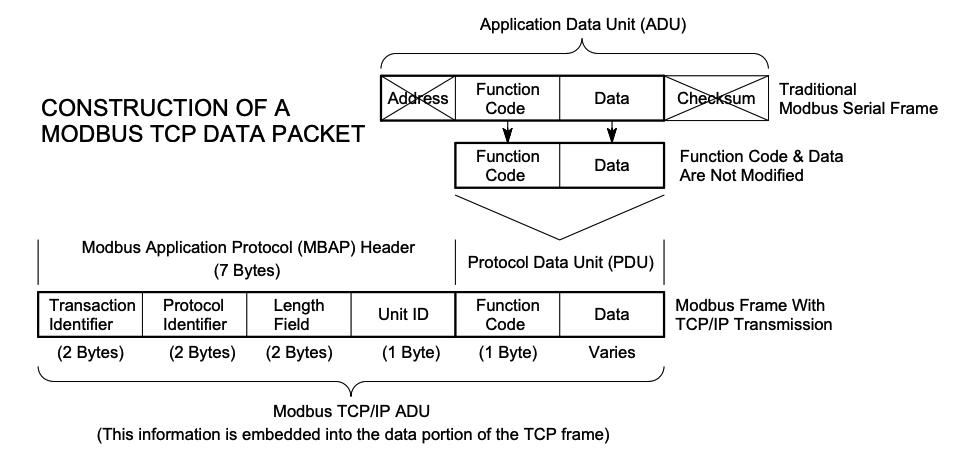
\includegraphics[width=10cm]{./graphics/Modbus-TCP-schema.png}
    \caption{Een grafische voorstelling van een Modbus TCP Data pakket. \autocite{Acromag2005}}
    \label{fig:modbus-data-pakket}
\end{figure}

\section{Data registers}
\label{sec:stand-van-zaken-dataregisters}

Aangezien het Modbus protocol gebruikt wordt om een verbinding te kunnen maken met de nodige apparatuur, moet ook bekend zijn welke data registers gebruikt moeten worden.\\

Om de metingen van de Siemens PAC2200 op te halen, wordt data register 65 uitgelezen, in dit register staat het totaal actief vermogen opgeslagen. Dit register is nodig om te weten of er energie opgewekt of aangekocht wordt. Nadat de waarde is opgehaald wordt er nog een berekening uitgevoerd om deze waarde in de juiste eenheid weer te geven.\\

Voor de laadpaal aan te sturen zijn er meerdere registers die gebruikt kunnen worden. Hier is een lijst van de data registers die carwash Clean Car belangrijk vindt:

\begin{itemize}
    \item Modbus Slave Max Current (1210) - Dit register wordt gebruikt om de maximale stroom, die de laadpaal mag gebruiken, te bepalen.
    \item Real Energy Consumed Sum (390) - Dit register geeft weer hoeveel energie de laadpaal op dat moment gebruikt.
    \item Mode 3 state (1201) - Dit register geeft de laadmodus van de laadpaal weer.
    \item Temperature (1102) - Dit register geeft de temperatuur van de laadpaal weer.
    \item Charge using 1 or 3 phases (1215) - Met dit register kan bepaald worden of de laadpaal in single- of 3-phase moet laden.
\end{itemize}

Bij deze registers, hebben registers 1210 en 1215 read/write privileges en registers 390, 1201 en 1102 read privileges, dit betekent dat registers 1210 en 1215 ook gebruikt kunnen worden om de laadpaal aan te sturen. Registers 390, 1201 en 1102 daarentegen kunnen enkel aangesproken worden om waarden uit te lezen.

\section{Authenticatie}
\label{sec:stand-van-zaken-authenticatie}

Er zijn verschillende manieren om een gebruiker te authenticeren in een applicatie. Zo zijn er ook verschillende authenticatie providers die gebruikt kunnen worden, maar aangezien de applicatie die gebouwd wordt voor Carwash Clean Car een interne applicatie is, wordt er gebruikgemaakt van een zelf geschreven authenticatie service. Deze service zal een e-mailadres en wachtwoord verwachten van de gebruiker. De applicatie zal enkel aanspreekbaar zijn voor het netwerk van de carwash, maar ook via een VPN-connectie met het netwerk van de carwash door middel van het ip adres van de webserver in te geven in de webbrowser. Als deze correct zijn, zal de service een token terugsturen naar de applicatie. Dit token wordt dan gebruikt om de gebruiker te authenticeren in de applicatie.

\section{Backend}
\label{sec:stand-van-zaken-backend}

Omdat er verschillende apparaten moeten aangestuurd worden, kan de vraag gesteld worden of dat deze allemaal rechtstreeks via de applicatie worden aangestuurd of dat er tussen de applicatie en de apparatuur, nog een extra service uitgewerkt wordt dat deze dan aanstuurt.\\

Een oplossing is dat er een backend met verschillende endpoints wordt opgesteld, zodat alle connecties met de apparaten makkelijk te testen vallen. De bedoeling is dan dat de applicatie de juiste waarden naar de juiste endpoints stuurt, zodat de apparaten niet rechtstreeks in contact met de applicatie komen te staan.\\

De endpoints van de backend zijn opgedeeld per apparaat. Dit wil zeggen dat alle requests voor het apparaat in kwestie naar de endpoint van het apparaat in kwestie worden doorgestuurd. Dit zijn de endpoints van de API:

\begin{itemize}
    \item \textbf{Authenticatie:}
          \begin{itemize}
              \item GET-request
                    \begin{itemize}
                        \item /login/:email
                    \end{itemize}
          \end{itemize}
    \item \textbf{Zonnepanelen:}
          \begin{itemize}
              \item GET-request
                    \begin{itemize}
                        \item /electricity/status
                    \end{itemize}
          \end{itemize}
    \item \textbf{Laadpaal:}
          \begin{itemize}
              \item GET-request
                    \begin{itemize}
                        \item /charging-station/max-current
                        \item /charging-station/energy-consumed-sum
                        \item /charging-station/mode
                        \item /charging-station/temp
                        \item /charging-station/charge/1-3-phases
                    \end{itemize}
              \item POST-request
                    \begin{itemize}
                        \item /charging-station/update-max-current
                        \item /charging-station/charge/update-1-3-phases
                    \end{itemize}
          \end{itemize}
    \item \textbf{Beluchtingssysteem:}
          \begin{itemize}
              \item GET-request
                    \begin{itemize}
                        \item /blower/status
                    \end{itemize}
              \item POST-request
                    \begin{itemize}
                        \item /blower/update-status
                    \end{itemize}
          \end{itemize}
\end{itemize}

\section{Front end}
\label{sec:stand-van-zaken-front-end}

De front end van de applicatie is een belangrijk deel van het volledige plaatje, omdat de eindgebruiker hier het meeste interactie mee heeft. Het framework dat gebruikt zal worden is React JS, omdat dit de voorkeur was van het bedrijf.\\

De reden dat dit de voorkeur is voor het bedrijf is omdat er veel documentatie en een actieve community over React JS beschikbaar is, dus als er een update nodig is aan het programma kan deze makkelijk door een derde partij doorgevoerd worden.

\section{Samenvatting}
\label{sec:stand-van-zaken-samenvatting}

In de literatuurstudie kwamen de belangrijkste spelers en methoden voor het besparen van energie aan bod. Zo is er een diepere kennis opgedaan over de spelers en methoden, met deze kennis kan er aan de proefopstelling gestart worden, om zo het project met succes af te kunnen ronden.\\

Zo is er te weten gekomen dat de 2 belangrijkste energieverbruikers de carwash en self-carwash zijn en dat de niet-dringende energieverbruikers bestaan uit de laadpaal, het beluchtingssysteem van het water en de industriële droogkast.\\

Als alle energieverbruikers geweten zijn, werden er methoden gezocht om de energiefactuur te verlagen. De 4 onderzochte methoden zijn: peak shaving, bidirectioneel laden van batterijen, het gebruik van algoritmen om de bedrijfsprocessen automatisch aan te sturen en energiebeheersystemen. Uit de onderzochte methoden bleek dat het gebruik van bidirectioneel laden nog niet kan toegepast worden in de carwash, aangezien de juiste infrastructuur nog niet aanwezig is. Zo is er gekozen om de andere 3 methoden toe te passen binnen de applicatie.\\

Na het bespreken van de methoden zijn de verschillende niet-dringende energieverbruikers en apparaten voor energieopbrengst besproken. In de hoofdstukken van de niet-dringende energieverbruikers is er dieper ingegaan op hoe deze apparatuur werkt en indien de apparatuur zelf niet slim aangestuurd kan worden, wat de benodigdheden zijn om dit wel te kunnen. Zo is er bij de laadpaal besloten dat de communicatie via het Modbus TCP/IP Slave protocol moet gebeuren. Bij de zonnepanelen werd de conclusie getrokken dat er 2 monitorsystemen in de carwash geïnstalleerd zijn, namelijk de Solarlog 1000 van Solarinventors en de Siemens PAC2200, maar dat de monitor van Siemens ook de aangekochte energie kan raadplegen en de monitor van Solarinventors deze fuinctionaliteit niet heeft. Voor het beluchtingssysteem van het water en de industriële droogkast aan te sturen zijn er smart plugs nodig. Aangezien er 1 smart plug aanwezig is in het bedrijf, dat geïnstalleerd staat bij het beluchtingssysteem, is besloten de industriële droogkast momenteel nog niet te integreren in de proefopstelling.\\

Het laatste deel van de literatuurstudie bevat de gebruikte protocollen, data registers, authenticatie van de applicatie, de backend en de front end. In het deel van de protocollen werd waargenomen dat enkel verschillende variaties van het Modbus protocol nodig zijn in de proefopstelling. In het hoofdstuk van de data registers werden de door het bedrijf gekozen data registers besproken en aangehaald wat deze juist deden. De authenticatie is zelf geschreven, omdat het een applicatie is die enkel beschikbaar is via het netwerk van de carwash. De conclusie van de backend bevatte alle endpoints van de API, zodat de webapplicatie niet rechtstreeks met de apparaten moet communiceren. In het deel van de front end werd de keuze van het gebruikte framework verantwoord.